\subsection{Services}
\label{services}

Mitglieder und Aufgaben:
\begin{itemize}
  \item
    Angelina Jellinek (Design der Webseite und Website Backend)
  \item
    Jan Arne Sparka (Integration von LUA und Server)
  \item
    Kevin Marc Trogant (Integration von Hardware und Server)
  \item
    Pascal Jochmann (Website Backend,Client-Server Kommunikation (Proto buffer))
  \item
    Tim Sikatzki (Website Backend und Datenbank)
\end{itemize}

\subsubsection{Aufbau}
Das gesamte Netzwerk ist über eine zentrales System realisiert. Die einzelnen 
Client kommunizieren nicht untereinander sonder alle mit dem Server der die Spielverwaltung übernimmt. 
Die Einstellungen der Spielparameter und die Darstellung des Punktestandes übernimmt eine Website die auf dem Server läuft. 
Auf dieser können die Spieler Dinge wie Spieleranzahl und Rundendauer festlegen außerdem meldet 
die Website dem Server den Start des Spiels. Zuletzt gibt es noch eine Datenbank zur Festhaltung des Punktestandes. 
Sie wird vom Server aktuell gehalten und von der Website auf einem Scoreboard dargestellt.

\subsubsection{Kommunikation}

Der Spielserver \texttt{services-server} nutzt einen eigenen Thread für die Kommunikation mit den Clients und
der Webseite. Clients und Server kommunizieren über BSD Sockets.
Als Alternative kam Googles gRPC in Frage. Dieses wurde verworfen, weil:
\begin{itemize}
    \item gRPC erlaubt Kommunikation nur in eine Richtung. Der Server kann nur dann Nachrichten an den Client verschicken,  wenn ein Request eingegangen ist.
    \item gRPC erlaubt nur einen Nachrichtentypen pro Kommunikationsrichtung. Da wir mehrere verschiedene Nachrichtentypen benötigen, hätten wir das Konzept eines Unions in gRPC nachbilden müssen.
\end{itemize}
Es wäre möglich gewesen Bibliotheken, zum Beispiel \href{http://think-async.com/Asio/WebHome}{boost.asio}, die eine einfachere Schnittstelle anbieten zu verwenden. Da wir zu dem Zeitpunkt, an dem wir entschieden haben die Socket API direkt zu verwenden, noch nicht genau wussten wie die Netzwerkkommunikation funktionieren würde, wollten wir uns möglichst viele Optionen offen halten. Außerdem hatten wir im Verlauf der Entwicklung mehrmals Probleme mit inkompatiblen Bibliotheksversionen, entweder durch andere APIs oder - wesentlich lästiger - durch unterschiedliches Verhalten. Deshalb waren wir später sehr zurückhaltend beim Einführen neuer Abhängigkeiten.

An die Datenbank ist der Server über die \href{https://dev.mysql.com/doc/connector-c/en/connector-c-introduction.html}{mysql c connector} Schnittstelle angebunden. Die Schnittstelle bietet eine relativ simple API: Zuerst verbindet sich das Programm mit dem MySQL Datenbankserver (entweder über TCP oder über Unix Sockets) und dann können beliebige SQL Anfragen als String an den Datenbankserver geschickt werden, der daraufhin Zeilenweise die Ergebnisse zurückliefert.
Diese Schnittstelle ist in einem C++ Singleton gekapselt \texttt{DatabaseConnection}, die Methoden für alle Anfragen
bereitstellt die der Server stellen muss (bswp \texttt{get\_runnable\_games()}). \newline
\newline
Der Thread für die Kommunikation führt in einer Endlosschleife folgende Schritte aus:
\begin{enumerate}
    \item Falls sich neue Clients verbunden haben: Lege die passenden Datenstrukturen an und setze den Status des Clients in der Datenbank auf verbunden.
    \item Hole eine Liste noch nicht beendeter Spiele von der Datenbank. Falls neue dazu gekommen sind, lege ein entsprechendes Objekt an.
    \item Frage den aktuellen Zustand aller Spiele die dem Server bekannt sind ab. Falls ein Spiel gestartet wurde, starte den entsprechenden Thread für die LUA API des Spiels.
    \item Sende den Spiellogik-Threadd aller neu beendeten Spiele eine Nachricht die diese dazu auffordert sich zu beenden.
    \item Empfange und Parse Nachrichten von Clients. (Siehe weiter unten)
    \item Zurück zu 1.
\end{enumerate}

Damit Spiel-Ereignisse an den Spieler kommuniziert werden können, kann die Spiellogik Funktionen auf dem Server aufrufen, die dafür sorgen das passende Nachrichten an die Clients gesendet werden. Dazu gibt es einen Nachrichtentyp in dem mittels eines Enums kodierte LED-Befehle enthalten sind. 

Das Nachrichtenformat ist mittels Google Protocol Buffers, Googles Lösung der Datenformatserialisierung umgesetzt. Dies ist eine sehr simple Lösung der Frage, wie wir die Nachrichten einheitlich und verständlich strukturieren. Protocol Buffers ist dabei im Vergleich zu den betrachteten alternativen wie XML am simpelsten mit dem wenigsten Overhead, während es trotzdem unseren Anforderungen genügt.\\
 Da Protocol Buffers jedoch selbst keine Möglichkeit
implementiert um aus einem empfangenem Byte-String den Nachrichtentyp zu rekonstruieren, wird vor jeder Nachricht
ein Header verschickt der den Nachrichtentyp und die Länge der Nachricht in Bytes enthält.
Die Nachrichten selbst können einfach mittels der Protocol-Buffers Bibliothek zu entsprechenden C++ Objekte geparst werden, die dann Nachrichtenfelder als \glqq Getter- und Setter-Funktionen\grqq \, verfügbar machen.

Die Kommunikation mit der Hardware-Komponente läuft über einen eigene Komponente (\texttt{services-client}) die auf den Spielgeräten ausgeführt wird. Diese empfängt Nachrichten von der Hardware-Schnittstelle über einen Unix-Socket, wandelt diese in das Services-Interne Format um und sendet sie dann über einen TCP Socket an den Server. Außerdem kümmert sich die Komponente darum in regelmäßigen Abständen (ca. 5 Sekunden) eine kurze \glqq Keep-Alive\grqq \, Nachricht an den Server zu senden um zu signalisieren das der Client noch verbunden ist und am Spielbetrieb teilnimmt. 
Eingehende Nachrichten vom Server, zum Beispiel um mittels der auf dem Gerät vorhandenden LEDs Treffer etc. anzuzeigen, werden vom Client empfangen und an die Hardware API weitergeleitet.\newline \newline
Da für ein Lasertag das Treffen von anderen Spielern von relativ hoher Bedeutung ist, soll hier noch kurz ausgeführt werden, was aus Sicht der Services-Komponente passiert wenn ein Spieler einen anderen trifft.

Zuerst erhält der Client eine Nachricht von der Hardware-API, die mitteilt das der Client getroffen wurde. In der Nachricht ist die ID des Clients enthalten, von der das Gerät getroffen wurde. Die eigene ID erhält der Client beim start. Diese beiden Informationen werden in eine sog. \glqq Hit-Message\grqq \, verpackt und an den Server gesendet. 
Der Server erhält die Nachricht, parst diese und sucht nach einem Spiel das beide Clients - Schießenden und Getroffenen - enthält. Findet er kein passendes Spiel, wird die Nachricht verworfen. Falls ein passendes Spiel gefunden wurde, werden die Client-IDs zu den entsprechenden Spieler-IDs aufgelöst (die Zuordnung ist pro Spiel eindeutig) und eine passende Nachricht an den entsprechenden Spiel-Thread geschickt.

\subsubsection{LUA API (services)}

Um Spielmodi zu beschreiben und sauber von den anderen Komponenten abzutrennen brauchten wir eine API. Die erste Entscheidung war zwischen LUA, c-Code und einer eigenen Spielmodus-DSL. Da unsere Spiellogikgruppe die Entscheidung für LUA traf und sogar schon einen funktionierenden Simulator für Spiele in sehr schneller sukzession herausbrachte, war diese Entscheidung für uns damit schnell getroffen.

Die LUA API auf services Seite war sehr schwierig einzubauen. Die erste Option war es die API als Singleton bereitzustellen, dies stellte sich aber sehr schnell als schlechter Ansatz heraus, da der Start einer weiteren Runde hierdurch zu einem komplizierten und unschönen Hack geworden wäre. Daher und da wir die Architektur für potentiel mehrere Spiele die Parallel laufen offen halten wollten, entschieden wir uns für den jetztigen Ansatz, die API läuft in einem eigenen Thread. 

Der Logik-Thread sammelt sich erstmal die relevanten Spieldaten zusammen, initialisiert dann die Felder auf welche LUA zugreift und geht dann in eine Event Loop über. In dieser Gameloop wird zuerst überprüft ob Schussnachrichten durchgereicht wurden, welche wiederum an LUA weitergereicht werden. Danach werden alle potentiellen Timer weitergetickt um die vergangene Zeit. Als letzte wird noch abgeprüft ob der Server uns ein AskedToExit Event schickt, welches mit Aufräumen und beenden des Spiels quittiert wird.

Der Hauptteil der API Arbeit auf der service Seite war die vorhandene Spiellogik API (den Simulator) an die real genutzte Hardware und Software anzubinden. Der Großteil der Input/Output Operationen wurde über unser Datenbankconnection Singleton umgeleitet. Das Scoreboard wird dabei permanent mitgeführt, wodurch Erweiterungen, wie z.B. spielerseitige Displays denkbar sind und was uns die Probleme von Score Serialisierung ignorieren lässt, da dieser sowieso von der Datenbank serialisiert wird. Da dann letztendlich die Relevanz eines Timers für LUA Skripte aufkam, welcher nicht den Logik-Thread vom Arbeiten abhält, haben wir einen einfachen Timer entwickelt der mit Funktionen Callbacks arbeitet. Die letzte Erweiterung der API war das hinzufügen der LED Events und der Abstraktion dieser in Funktionen, die Teil der LUA API wurden.

Die services Seite der LUA API hatte als Hauptproblem, das sie aufgrund der sehr zentralen Stellung (Verknüpfung von 3 Komponenten), sehr viele Abhängigkeiten hatte und sehr schwierig zu testen war. Dies ist dem Projekt letztendlich zum Verhängnis geworden, da wir in der Interaktion dieser vier Komponenten einen Fehler haben, den wir bisher noch nicht lokalisieren konnten. Das Debugging ist auf Grund von LUA auch nur sehr begrenzt möglich und wird uns noch einiges an Aufwand einbringen.
\shorthandoff{"}
\subsubsection{Website}

Unsere Website bildet das Herzstück in der Interaktion zwischen dem Nutzer und der Software. Sie gibt ihm die Möglichkeit, die Konfigurationen für das Spiel einzustellen, wie zum Beispiel die Anzahl der Teams, dem Spielmodus und den Spielgeräten Namen zuzuteilen. Außerdem haben die Spieler durch sie die Möglichkeit, ihre Leistungen während des Spiels in Echtzeit einsehen zu können.\\\\
Zur Entwicklung der Website haben wir "Flask" benutzt, ein Webframework auf Python-Basis. Wir haben uns für dieses Framework entschieden, da es zunächst sehr leicht zu benutzen ist und uns gleichzeitig alles geboten hat, um die erwarteten Funktionalitäten der Website implementieren zu können, wie zum Beispiel ein MySQL-Package, welches wir zur Interaktion zwischen Webapplikation und Datenbank benutzt haben.
Um die oben genannten Funktionen gewährleisten zu können, besteht unsere Webapplikation aus mehreren HTML-Seiten.\\\\
Die erste Seite (Abb.3) ist der Kern der Website. Sie wird benutzt, um das eigentliche Spiel zu erstellen. Nicht nur nimmt sie die eingegebenen Daten der Spieler auf, sondern überträgt die Einstellungen direkt auf die Datenbank und erstellt dort direkt Einträge, die für das Scoreboard relevant sind. In der Sektion Datenbank werden die Einträge und Tabellen genauer erläutert. Die möglichen Einträge der Spielernamen sind hierbei abhängig von der Anzahl der verbundenen Clients. Sind nur drei Clients zum Server verbunden, so können wir auch nur drei Namen zuweisen.
Auch die Spielmodi, die ausgewählt werden können, werden dynamisch erstellt. Hierbei wird aus einem Ordner ausgelesen, in dem die Lua-Skripte abgelegt werden können. Die Teams werden von der Webapplikation mithilfe von einer Modulo-Operation, abhängig von der Teamanzahl, automatisch zugeteilt. Es ist also \\\\
Sobald ein Spiel gestartet wird, leitet die Seite auf das Scoreboard weiter.\\ Das Scoreboard zieht sich seine Einträge direkt aus der Datenbank und aktualisiert dieses asynchron unter der Verwendung von jQuery und ajax. Es stellt die Einträge in Form von Tabellen da, hierbei gibt es eine Tabelle die Spieler und eine Tabelle für die Teams (Abb.4). Auf der Seite haben wir dann die Möglichkeit, das Spiel manuell zu pausieren oder auch zu beenden. Wenn die Dauer einer Runde ausgelaufen ist, wird das Spiel automatisch in den pausierten Zustand gesetzt. Wir können nun jederzeit eine mithilfe des Links "Spiel fortfuehren" Eine neue Runde starten bzw. das pausierte Spiel weiterspielen.\\
Der Link "Spiel beenden" funktioniert dementsprechend genauso, allerdings ist es danach nicht mehr möglich, das Spiel weiterzuführen. Der Nutzer dann danach auf einen Button klicken, um zurück zur Startseite zu gelangen und ein neues Spiel zu starten .\\\\
Insgesamt ist die Webapplikation seitens Funktionalität vollständig. Es könnten noch Verbesserungen hinsichtlich der Anzeige der verschiedenen Dateifragmente und der Effizienz der Anzeige des Scoreboards gemacht werden.


\subsubsection{Style}

\begin{figure}[htb]
	\begin{center}
		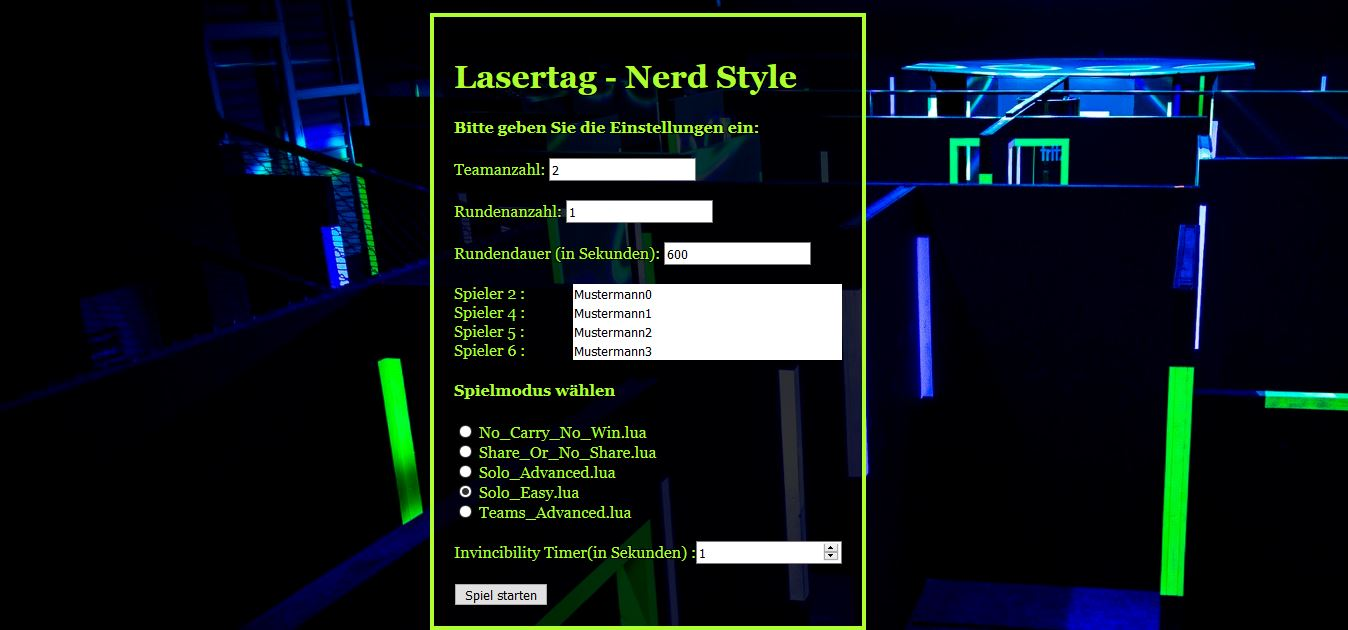
\includegraphics[width=0.75 \textwidth]{websitemenue.JPG}
		\caption{Startseite}
	\end{center}
\begin{center}
	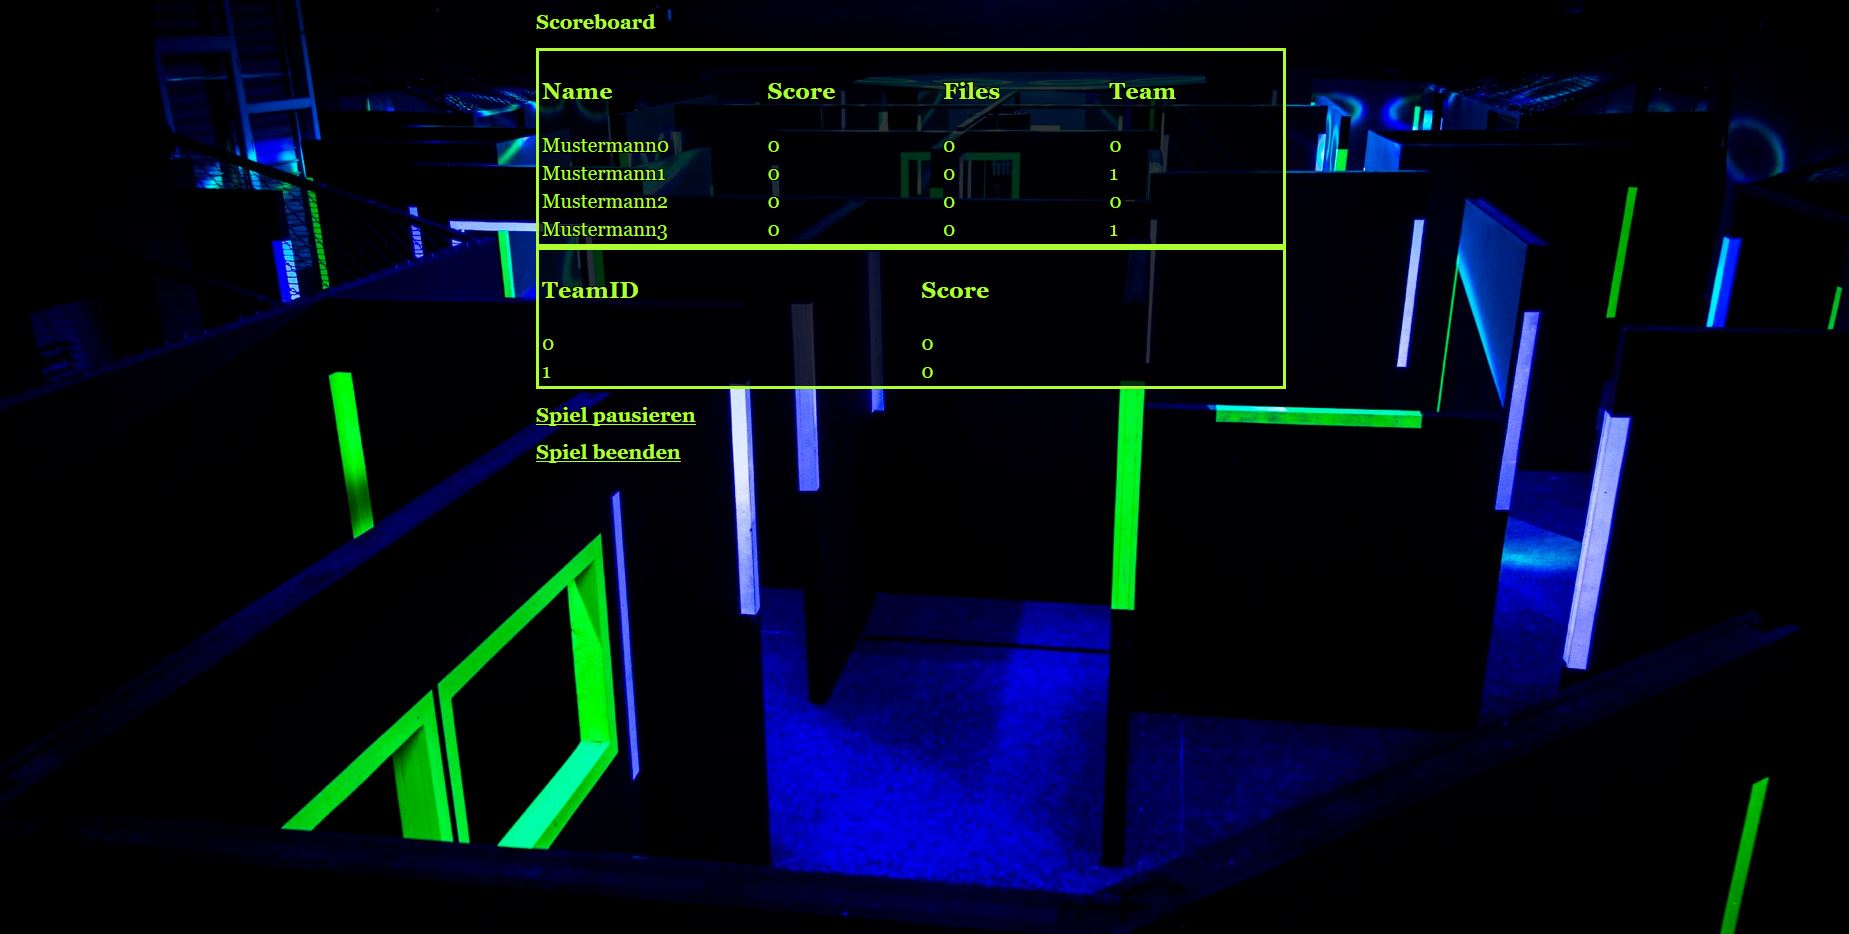
\includegraphics[width=0.75 \textwidth]{scoreboardteams.JPG}
	\caption{Scoreboard mit Teams}
\end{center}
\end{figure}
%\begin{figure}[b]
	
%\end{figure}

Viele Styleformatierungen sind auf der Scoreboardseite genau wie auf der Startseite. Es gibt jedoch auch noch einige Besonderheiten. Da sich das Scoreboard regelmäßig aktualisiert mussten wir die Links zu der gestoppten und pausierten Seite so designen, dass er im „Originalzustand“ und „angeklicktem Zustand“ genau gleich aussieht und nicht als Link erkennbar ist.
Das Aussehen der Website ist  dynamisch gestaltet. Die Größe des Scoreboards passt sich individuell an die Anzahl der Einträge an. Auch die Box passt sich dynamisch an die Einträge an. Gleichzeitig gibt es auch nur ein extra Scoreboard für Teams, wenn es Teams auch wirklich gibt.\\ Sowohl der Hintergrund, als auch die Schriftart und die Farben sind so gewählt, dass sie zum Thema Lasertag und Nerd Style passen. 
Die Schrift ist in grün gehalten, damit ein guter Kontrast zwischen Hintergrund und Text entsteht. Der Hintergrund dieser Textfelder hat eine leicht schwarze Transparenz bekommen, damit die grüne Schrift auch auf helleren Stellen des Hintergrunds der Website gut lesbar ist. Alle Textfragmente einer Seite befinden sich in einer Box, um die Position auf der Seite bestimmen zu können, ohne kleine Unregelmäßigkeiten der Einrückungen zu bekommen. Es stehen mehrere Schriftarten zur Auswahl, von denen die erste angewendet wird, die dargestellt werden kann. Hier handelt es sich um die Schriftarten Georgia und Times New Roman. Das Design dunkel genug und wenig belastend für die Augen, um es in einer dunklen Halle auf eine Leinwand zu übertragen, ohne dabei die Spieler von ihrem Spiel abzulenken. \\\\


\subsubsection{Datenbank}
\begin{figure}[htb]
	\begin{center}
		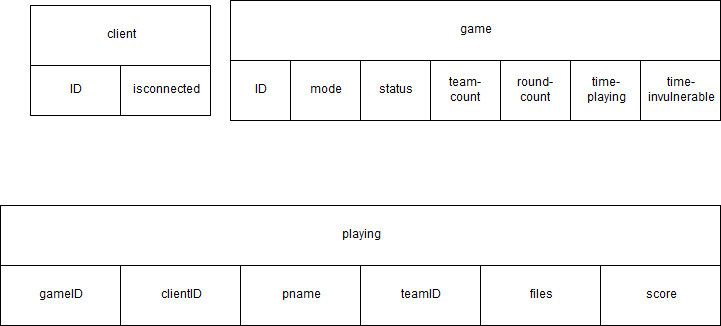
\includegraphics[width=0.8 \textwidth]{Databasestrucb.png}
		\caption{Datenbankstruktur}
	\end{center}
\end{figure}
Unsere Datenbank ist die ermöglichte uns die Interaktion innerhalb der services-Gruppe. Wir haben uns für eine Datenbank entschieden, da wir eine Spielhistorie aus den vergangenen Spielen erstellen wollten. Gleichzeitig bot sich die Datenbank auch für die Darstellung des Scoreboard an, da die SQL Anfragen für eben dieses sehr trivial waren.\\\\
Um die Fehlerquelle einer Datenbank in Forvm einer Datei zu umgehen, haben wir uns nach einiger Zeit dafür entschieden von SQLite auf MySQL, als Datenbankmanagementsystem, umzusteigen.\\\\
%Abbildung mit Tabellen hier einfügen

In Abbildung 5 sehen wir den Aufbau unserer Datenbank. Wie wir sehen können, ist sie in drei Tabellen unterteilt.\\
Die client - Tabelle ist relevant für das Anzeigen der möglichen Eingabefelder für die Spielernamen im Menü der Website. Hierbei wird unterschieden, ob ein Client mit dem Server verbunden ist oder nicht.\\\\
Die game - Tabelle ist vorallem interessant für die LUA API, da sie die Einträge enthält, die von dem Spieler vor Beginn des Spieles mithilfe des Menüs übergeben werden, wie zum Beispiel der Spielmodus und die Rundendauer. Gleichzeitig beinhaltet die Tabelle auch den Status, den das jeweilige Spiel zu jeder Zeit hat. Dieser Status wird von allen Parteien benutzt: die LUA API muss das Spiel nach Überschreiten der Rundendauer pausieren oder es beenden, die Netzwerkkommunikation muss bei einem gestoppten Spiel aufhören, Nachrichten weiterzuschicken, damit keine Punkte während eines pausierten oder beendeten Spieles verteilt werden.\\\\\\
Die "playing" - Tabelle wird für unsere Historie und gleichzeitig der Darstellung des Scoreboards benutzt. Sie teilt jedem Spieler eine gameID, den jeweiligen Score, die Dateifragmente usw. zu und macht es möglich die Tabelle nach der gameID zu sortieren um einzelne Spiele wieder einsehen zu können.

\shorthandon{"}
\subsubsection{Debugging}

Um Fehler zu finden und das Verhalten des Systems nachvollziehen zu können, geben sowohl Client als auch Server Log-Ausgaben auf \texttt{stderr} aus. Da beide von systemd gestartet werden, können diese Log-Ausgaben auch mit den üblichen Systemd-Kommandos angezeigt werden.
